\documentclass{assignment}
\ProjectInfos{高等热力学与统计物理}{PHYS2110}{2020-2021学年第二学期}{习题 VI}{截止时间:2021. 4. 13(周二)}{陈稼霖}{45875852}

\begin{document}
\begin{prob}
    计算 Maxwell 分布下的最可几速度,平均速度和速度分布的宽度,即
    \begin{align}
        \Delta v\equiv\sqrt{\langle(v-\langle v\rangle)^2\rangle}
    \end{align}
    将结果用绝对温度和分子质量表达,并算出氢气和氧气以上各量在室温下的数值.
\end{prob}
\begin{sol}
    
\end{sol}

\begin{prob}
    由同一种分子组成的理想气体被隔膜分成两部分. 每部分的体积,粒子数和温度如右图所示. 假设隔膜左右温度相同,但密度不同,且系统与外界热绝缘. 证明隔膜撤掉后气体的熵增加.
    \begin{figure}[htb]
        \centering
        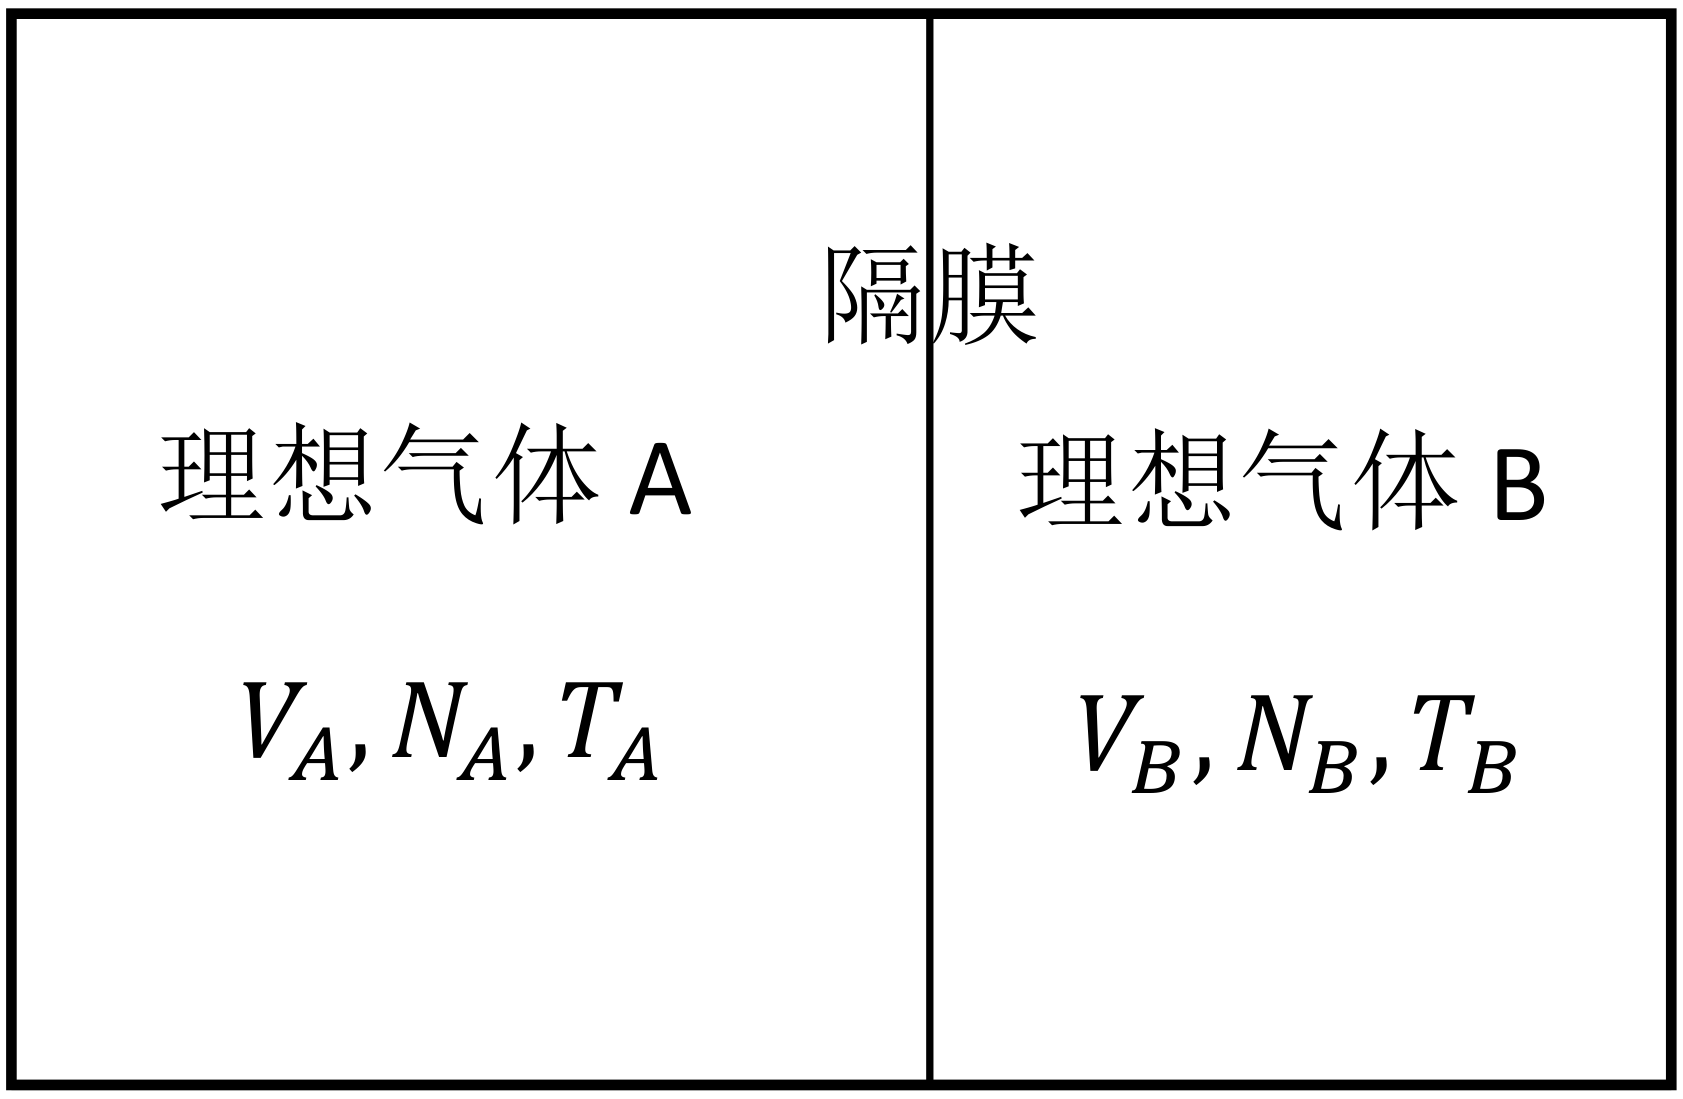
\includegraphics[width=.4\columnwidth]{A6-P2.png}
    \end{figure}
\end{prob}
\begin{pf}
    隔膜撤掉后气体的熵的改变量为
    \begin{align}
        \label{2-DeltaS}
        \notag\Delta S=&S_2-S_1=S_2-S_{1A}-S_{1B}=(N_A+N_B)k\ln\frac{V_A+V_B}{N_A+N_B}-N_Ak\ln\frac{V_A}{N_A}-N_Bk\ln\frac{V_B}{N_B}\\
        =&(N_A+N_B)k\left[\ln\frac{V_A+V_B}{N_A+N_B}-\frac{N_A}{N_A+N_B}\ln\frac{V_A}{N_A}-\frac{N_B}{N_A+N_B}\ln\frac{V_B}{N_B}\right].
    \end{align}
    函数
    \begin{align}
        f(x)=\ln x
    \end{align}
    的二阶导
    \begin{align}
        f''(x)=-\frac{1}{x^2}<0,
    \end{align}
    故 $f(x)$ 为上凸函数. 式 \eqref{2-DeltaS} 中括号内的部分可写作
    \begin{align}
        \notag&\ln\frac{V_A+V_B}{N_A+N_B}-\frac{N_A}{N_A+N_B}\ln\frac{V_A}{N_A}-\frac{N_B}{N_A+N_B}\ln\frac{V_B}{N_B}\\
        =&f\left(\frac{N_A}{N_A+N_B}\frac{V_A}{N_A}+\frac{N_B}{N_A+N_B}\frac{V_B}{N_B}\right)-\frac{N_A}{N_A+N_B}f\left(\frac{V_A}{N_A}\right)-\frac{N_B}{N_A+N_B}f\left(\frac{V_B}{N_B}\right).
    \end{align}
    其中 $\frac{N_A}{N_A+N_B}+\frac{N_B}{N_A+N_B}=1$. 根据上凸函数的性质,
    \begin{gather}
        f\left(\frac{N_A}{N_A+N_B}\frac{V_A}{N_A}+\frac{N_B}{N_A+N_B}\frac{V_B}{N_B}\right)>\frac{N_A}{N_A+N_B}f\left(\frac{V_A}{N_A}\right)+\frac{N_B}{N_A+N_B}f\left(\frac{V_B}{N_B}\right),\\
        \Longrightarrow\ln\frac{V_A+V_B}{N_A+N_B}-\frac{N_A}{N_A+N_B}\ln\frac{V_A}{N_A}-\frac{N_B}{N_A+N_B}\ln\frac{V_B}{N_B}\geq 0.
    \end{gather}
    从而
    \begin{align}
        \Delta S>0,
    \end{align}
    即隔膜撤掉后气体的熵增加.
\end{pf}

\begin{prob}
    在高温条件下,即
    \begin{align}
        \varepsilon\equiv\frac{\hbar^2}{2IkT}\ll 1
    \end{align}
    证明双原子气体的转动配分函数
    \begin{align}
        q_r=\omega\left[\frac{1}{\varepsilon}+\frac{1}{3}+\frac{1}{15}+O(\varepsilon^2)\right]
    \end{align}
    和每个分子平均转动动能
    \begin{align}
        u_r=kT\left[1-\frac{1}{3}\varepsilon-\frac{1}{45}\varepsilon^2+O(\varepsilon^3)\right]
    \end{align}
    其中 $\omega$ 为核自旋的简并度.
    \begin{align}
        \omega=\left\{\begin{array}{ll}
            (2s_A+1)(2s_B+1),&AB\text{型}\\
            \frac{1}{2}(2s_A+1)^2,&AA\text{型}
        \end{array}\right.
    \end{align}
    提示:可用 Eular-Maclaurin 公式计算修正项.
\end{prob}
\begin{pf}

\end{pf}
\end{document}